\chapter{Realizability Problems for Weighted Trees}
In figure \ref{fig:hexagonOutline5LayerSmall.pdf}, we have a set of unit radius disks (circles) arranged in a manner that outlines regular, concentric hexagons.
\begin{figure}[!htbp]
\begin{center}
\includegraphics{graphics/hexagonOutline5LayerSmall.pdf}
\caption{A contact graph that resembles the shape of concentric hexagons.}\label{fig:hexagonOutline5LayerSmall.pdf}
\end{center}
\end{figure}
\begin{prob}[Appoximating Polygonal Shapes with Contact Graphs]\label{problem:ApproxShapesWithContactGraphs}
For every $\epsilon >0$ and polygon $P$, there exists a contact graph $G = (V,E)$  such that the Hausdorff distance $d(P,G) < \epsilon$
\end{prob}

Recall problems (\ref{problem:UnorderedContactGraph}) and (\ref{problem:OrderedContactGraph}): given a positive weighted tree, $T$, is $T$ the (ordered) contact graph of some disk arrangement where the radii are equal to the vertex weights.  For now, we'll focus on a particular family of this problem space where the weighted trees can be realized as a \textit{snowflake}. For $i \in \bbN$, the construction of the snowflake tree, $S_i$, is as follows:
\begin{itemize}
\item Let $v_0$ be a vertex that has six paths attached to it: $p_1$, $p_2$, $\dots$, $p_6$.  Each path has $i$ vertices.
\item For every other path $p_1$, $p_3$, and $p_5$: 
	\begin{itemize}
		\item 	Each vertex on that path has two paths attached, one path on each side of $p_k$.
		\item	The number of vertices that lie on the path attached to the $j^\text{th}$ vertex of $p_k$ is $i-j$.
	\end{itemize}
\end{itemize}
\begin{figure}[!htbp]
\begin{center}
\includegraphics{graphics/snowflakeOutline5LayerSmall.pdf}
\caption{The same contact graph as in figure \ref{fig:hexagonOutline5LayerSmall.pdf} overlayed with the a perfectly weighted snowflake tree.}\label{fig:snowflakeOutline5LayerSmall.pdf}
\end{center}
\end{figure}

A \textit{perfectly weighted snowflake tree} is a snowflake tree with all vertices having weight $\frac{1}{2}$.  A \textit{perturbed snowflake tree} is a snowflake tree with all vertices having weight of 1 with the exception of $v_0$;  in a perturbed snowflake tree, $v_0$ will have a weight of $\frac{1}{2} + \gamma$.  For our analysis, all realizations of any snowflake, perfect or perturbed, shall have $v_0$ fixed at origin.  This is said to be the canonical position under Hausdorff distance of the snowflake tree.   

\paragraph{Perfectly Weighted Snowflake Tree.}

Consider the graph of the triangular lattice with unit distant edges:
\begin{eqnarray*}
V &=& \left\lbrace a\cdot (1,0) + b \cdot \left(\frac{1}{2},\frac{\sqrt{3}}{2}\right) : a,b \in \bbZ \right\rbrace\\
E &=& \left\lbrace \left\lbrace u,v \right\rbrace : \vert\vert u-v \vert\vert = 1 \text{ and } u,v \in V\right\rbrace
\end{eqnarray*}
The following graph, $G=(V,E)$ is said to be the \textit{unit distance graph} of the triangular lattice.  We can show that no two distinct edges of this graph are non-crossing.  First suppose that there were two distinct edges that crossed, $\left\lbrace u_1,v_1 \right\rbrace $ and $\left\lbrace u_2,v_2 \right\rbrace$.  With respect to $u_1$, there are 6 possible edges corresponding to it, with each edge $\frac{\pi}{3}$ radians away from the next.  Neither edge crosses another; and so we have a contradiction that there are no edge crossings with $\left\lbrace u_1,v_1 \right\rbrace $.  


The perfectly weighted snowflake tree that is a subgraph over the \textit{unit distance graph}, $G=(V,E)$, of the triangular lattice.  To show this, for any $S_i$, fix $v_0 = 0 \cdot \cdot (1,0) + 0 \cdot \left(\frac{1}{2},\frac{\sqrt{3}}{2}\right)=\lr{0,0} \in V$ at origin.  Next consider the six paths attached from origin.  Fix each consecutive path $\frac{\pi}{3}$ radians away from the next such that the following points like on the corresponding paths: $\lr{1,0} \in p_1, \lr{\frac{1}{2} ,\frac{\sqrt{2}}{3}} \in p_2,\lr{-\frac{1}{2}\p_4,\frac{\sqrt{3}}{2}} \in p_3, \lr{-1,0} \in p4, \lr{-\frac{1}{2},-\frac{\sqrt{3}}{2}}\in p_5,\lr{\frac{1}{2},-\frac{\sqrt{3}}{2}}\in p_6$.  For $S_i$, there are $i$ vertices on each path.  

We define the six paths from origin as follows:
\begin{eqnarray*}
p_1 &=& \set{a\cdot\lr{1,0} = \vec{v}}{a \in \bbR^+}\\
p_2 &=& \set{a\cdot\lr{\frac{1}{2},\frac{\sqrt{3}}{2}} = \vec{v}}{a \in \bbR^+}\\
p_3 &=& \set{-a\cdot \lr{1,0} + a \cdot \lr{\frac{1}{2},\frac{\sqrt{3}}{2}} = a\lr{-\frac{1}{2},\frac{\sqrt{3}}{2}} = \vec{v}}{a \in \bbR^+}\\
p_4 &=& \set{a \cdot \lr{-1,0} = \vec{v}}{a \in \bbR^+}\\
p_5 &=& \set{a \cdot \lr{-\frac{1}{2},-\frac{\sqrt{3}}{2}}  = \vec{v}}{a \in \bbR^+}\\
p_6 &=& \set{ a\cdot \lr{1,0} - a \cdot \lr{\frac{1}{2},\frac{\sqrt{3}}{2}}= a \cdot \lr{\frac{1}{2}, -\frac{\sqrt{3}}{2}}}{a \in \bbR^+} 
\end{eqnarray*}
For $S_i$ there exists $i$ vertices on each path.  We shall denote the $i^\text{th}$ vertex on the $j^\text{th}$ path as $v_{j,i}$.  For each path defined above, the paths are defined as a set of vectors, $\vec{v} = a \cdot \vec{p}$  for some $a \in \bbR^+$ and $\vec{p} \in \bbR^2$.  By setting $a = 1,2,\dots, i$, we obtain points that are contained in $V$.  For $j = 1,3,5$ and $l = 1,..., i$, there exists two paths attached to each vertex $v_{j,l}$.  For $S_i$, each path attached to the $k^\text{th}$ vertex of $p_j$, there are $i-k$ vertices.  We will need to show that each of the $i-k$ vertices on each corresponding path are also in $V$.

The triangular lattice is symmetice under rotation about $v_0$ by $\frac{\pi}{3}$ radians.  For each vertex $v_{1,l}$ for $l=1,2,..., i-k$, we place two paths from it; the first path $\frac{\pi}{3}$ above $p_1$ at $v_{1,l}$ and $\frac{-\pi}{3}$ below $p_1$ at $v_{1,l}$ and call these paths $p_{1,l}^+$ and $p_{1,l}^-$ respectively.  With respect to $v_{1,l}$, one unit along $p_{1,l}^+$ is a point on the triangular lattice and similarly so on $p_{1,l}^-$.  Continuing the walk along these paths, unit distance-by-unit distance, we obtain the next point corresponding point on the the triangular lattice up to $i-k$ distance away from $v_{1,l}$.  This shows that each of the $i-k$ vertices on $p_{1,l}^-$ and $p_{1,l}^+$ are in $V$.  By rotating all of the paths along $p_1$ by $\frac{2\pi}{3}$ and $\frac{4\pi}{3}$, we obtain the the paths along $p_3$ and $p_5$ respectively, completing the construction.

\paragraph{Perturbed Snowflake Tree.}

The perturbed snowflake follows the construction of the perfect snowflake with the exception of $v_0$ having weight $\frac{1}{2} + \gamma$ where $\gamma > 0$.
A perturbed snowflake realization has some distinct qualities from perfect snowflake realizations.  
The angular relationships between adjacent vertices may vary; the distance between adjacent and neighboring vertices may vary as well.

%Consider a perturbed snowflake with six unit weight vertices having an edge to $v_0$, each unit weighted vertex lying on one distinct path $p_1, \ldots, p_6$.


\begin{minipage}{\linewidth}
\begin{center}
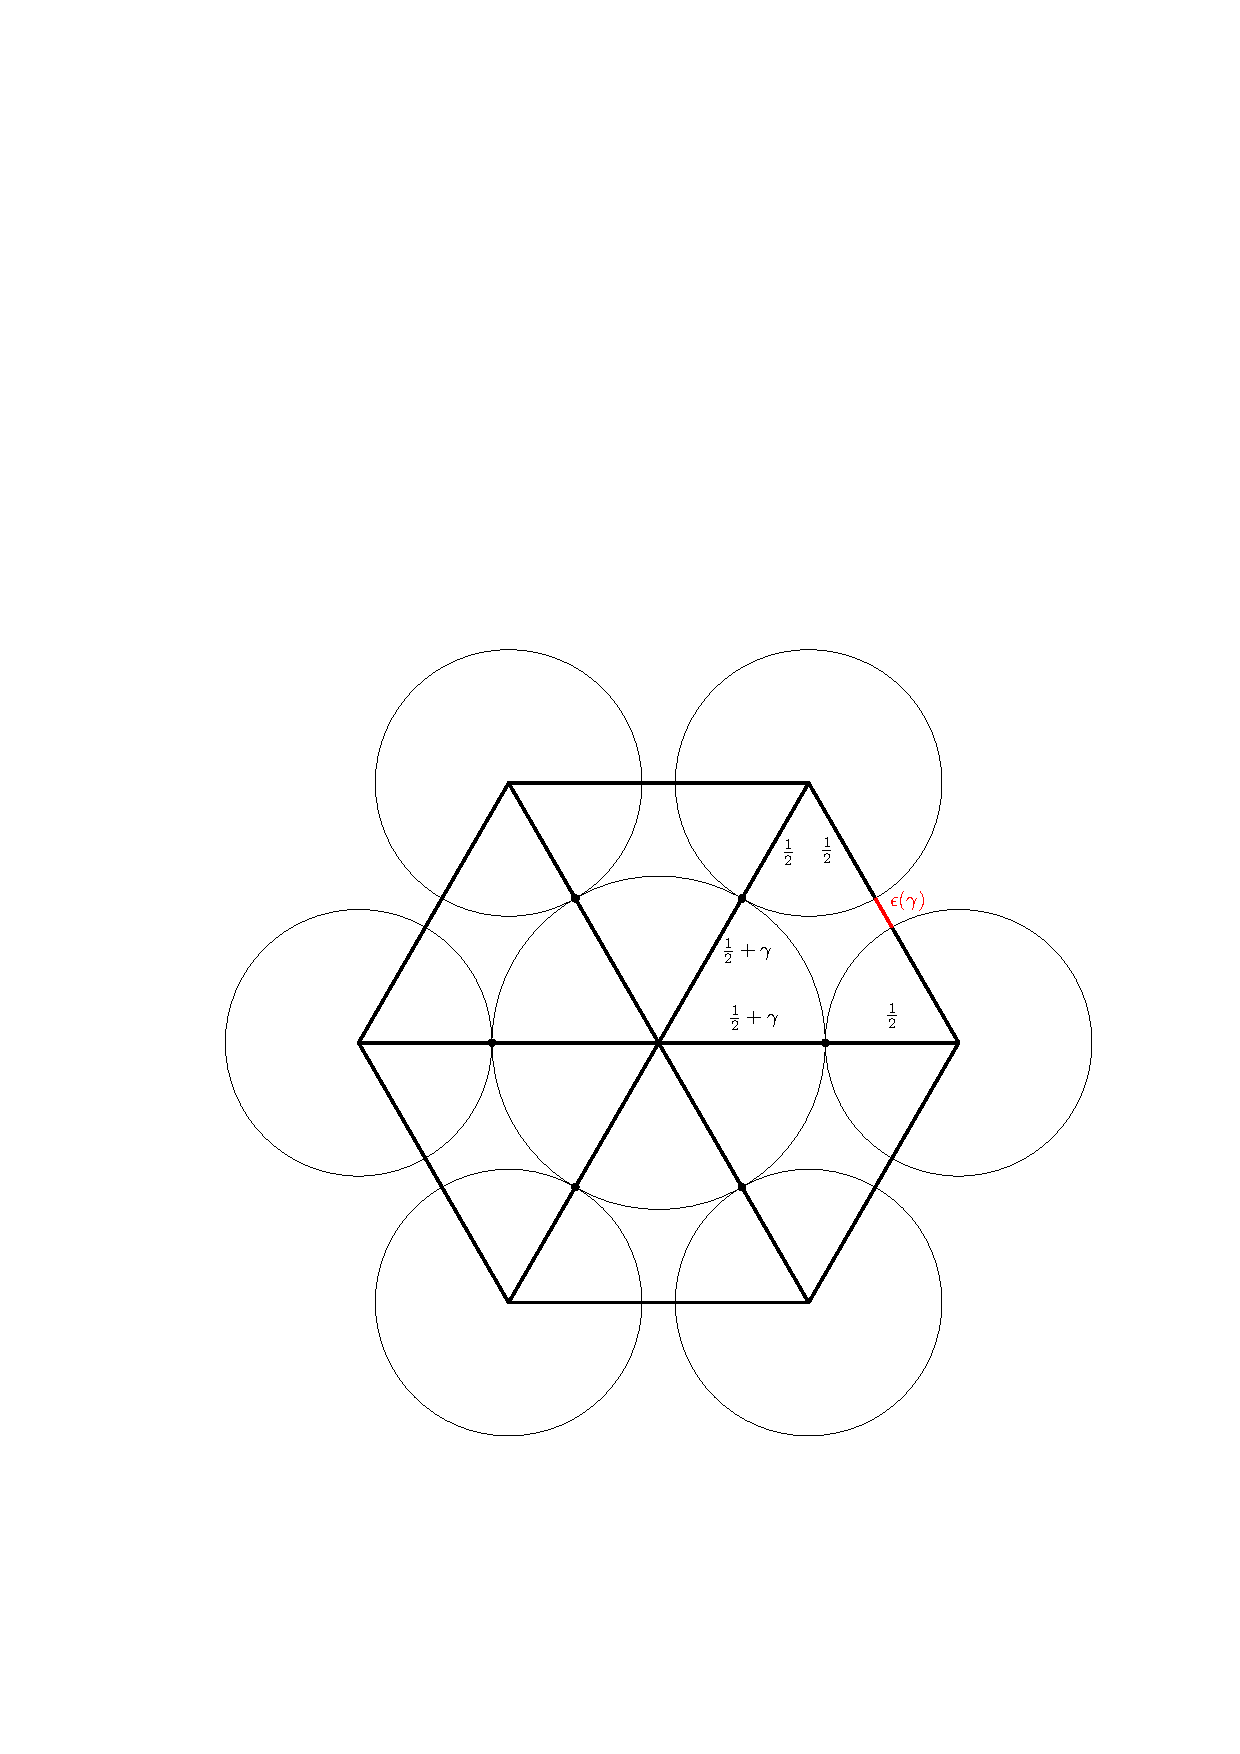
\includegraphics[width=.33\columnwidth]{graphics/modifiedContactGraph.pdf}
\captionof{figure}{A disk arrangement from a perturbed snowflake with 6 unit disks around a central disk with radius $\frac{1}{2} + \gamma$.}\label{fig:modifiedContactGraph.pdf}
\end{center}
\end{minipage}

In Figure \ref{fig:modifiedContactGraph.pdf}, we have a realization of disk arrangement from a perturbed snowflake.
In a disk arrangement of a perfect snowflake, the disks around the central disk contact the adjacent disks.
The disk arrangement from the perturbed snowflake does not have this quality.  
Figure \ref{fig:modifiedContactGraph.pdf} shows a gap $\epsilon(\gamma)$ between the disks around the central disk.  
This gap is formed from the perturbed weight $\frac{1}{2} + \gamma$ of the central disk.  


 \section{On the Decidability of Problem \ref{problem:UnorderedContactGraph}}
\begin{proof} 
Consider a $k \times (\sqrt{3}k)$ rectangle section of a triangular lattice, and place disks of radius 1 at each grid point as in Fig. ?????. 
The contact graph of these disks contains 2-cycles. 
Consider the spanning tree $T$ of the contact graph indicated in Fig. ????. 
The tree $T$ decomposes into paths of collinear edges: $T$ contains two paths along the two main diagonals, each containing $2k - 1$ vertices; all other paths have an endpoint on a main diagonal. 
 We now modify the disk arrangement to ensure that its contact graph is $T$. 
 The disks along the main diagonal do not change. 
 We reduce the radii of all other disks by a factor of $1 - k^{-3}$ (as a result, they lose contact with other disks), and then successively translate them parallel in the direction of the shortest path in $T$ to the main diagonal until the contact with the adjacent disk is reestablished. 
 The Hausdorff distance between the union of these disks and the initial $k \times (\sqrt{3}k)$ rectangle is clearly less than 1.
 However, the contact tree $T$ with these radii no longer has a unique realization (small perturbations are possible). 
 To show stability, we argue by induction on the hop distance from the central disk. 
 There are $O(i)$ disks at i hops from the central disk, most one which have radius $(1-k^{-3}) \frac{1}{2}$.
 Since all radii are 1 or $(1-k^{-3}) \frac{1}{2}$,the six neighbors of the central disk can differ from the regular hexagon by at most $O(k )$. 
 Similarly, the disks at $i$ hops from the center be off from the triangular grid pattern by $O(i2^{k-3})$, for $i = 1,2,\dots,k$.
\end{proof}


% Recall that problem (\ref{problem:UnorderedTree}) states: given a positive weighted tree, $T$, is $T$ the contact graph of some disk arrangement where the radii are equal to the vertex weights?  

% \begin{proof}
% Suppose we are given a positive weighted tree, $T = \lr{V_1,E_1}$.  By the Disk Packing Theorem, there is a disk arrangement in the plane, $D$, whose contact graph, $G=\lr{V_2,E_2}$ is isomorphic to $T$.  We need to so that $G=T$ and the radii of the disks in $D$ are equal to the vertex weights of $T$.

% To show that $G=T$, we need to show that $V_1=V_2$ and $E_1=E_2$.  

% To show that the radii of the disks in $D$ are equal to the vertex weights of $T$, we first consider ....  
% \end{proof}

% Related Previous Work. Polygonal linkages (or body-and-joint frameworks) are a gen-
% eralization of classical linkages (bar-and-joint frameworks) in rigidity theory. A linkage
% is a graph G = (V, E) with given edge lengths. A realization of a linkage is a (crossing-
% free) straight-line embedding of G in the plane. Bhatt and Cosmadakis [3] proved that
% the realizability of linkages is NP-hard. Their “logic engine” method [11, 13, 15, 18],
% has become a powerful tool in graph drawing. The logic engine is a graph composed
% of rigid 2-connected components, connected by cut vertices (hinges). The two possi-
% ble realizations of each 2-connected component (that differ by a single reflection) rep-
% resent the truth assignment of a binary variable. This method does not applicable to
% the oriented version of the realizability, where the circular order of the neighbors of
% each vertex is part of the input. Cabello et al. [6, 14] proved that the realizability of 3-
% connected linkages (where the orientation is unique by Steinitz’s theorem) is NP-hard,
% but efficiently decidable for near-triangulations [6, 12].
% Note that every tree linkage can be realized in R2 (with almost collinear edges).
% According to the celebrated Carpenter’s Rule Theorem [9, 21], every realization of a
% path (or a cycle) linkage can be continuously moved (without self-intersection) to any
% other realization. In other words, the realization space of such a linkage is always con-
% nected. However, there are trees of maximum degree 3 with at few as 8 edges whose
% realization space is disconnected [2]; and deciding whether the realization space of a
% tree linkage is connected is PSPACE-complete [1]. (Earlier, Reif [20] showed that it is
% PSPACE-complete to decide whether a polygonal linkage can be moved from one re-
% alization to another among polygonal obstacles in R3.) Cheong et al. [7] considers the
% “inverse” problems of introducing the minimum number of point obstacles to reduce
% the configuration space of a polygonal linkage to a unique realization.
% Connelly et al. [10] showed that the Carpenter’s Rule Theorem generalizes to certain
% polygonal linkages, which are obtained by replacing the edges of a path linkage with
% special polygons called (slender adornments). Our Theorem 1 indicates that if we are
% allowed to replace the edges of a path linkage with arbitrary convex polygons, then
% deciding whether the realization space is empty or not is already NP-hard.
% Recognition problems for intersection graphs of various geometric object have a
% rich history [18]. Breu and Kirkpatrick [5] proved that it is NP-hard to decide whether
% a graph G is the contact graph of unit disks in the plane (a.k.a. recognizing coin graphs
% is NP-hard). A simpler proof was later provided via the logic engine [13]. It is also NP-
% hard to recognize the contact graphs of pseudo-disks [18] and disks of bounded radii [4]
% in the plane, and unit disks in higher dimensions [17, 18]. All these hardness reductions
% produce graphs of high genus, and do not apply to trees. Note that the contact graphs
%  of disks (of arbitrary radii) are exactly the planar graph (by Koebe’s circle packing
%  theorem), and planarity testing is polynomial. Consequently, every tree is the contact
%  graph of disks of some radii in the plane.


%My goals for next week are as follows:
%1) Clean up chapter 1.  This will happen over the next several weeks.
%2) Continue section 2.3
%3) Add graphics to epsilon-approximation definition to facilitate the explanation.
%4) Anything else  I have time for.



% $\overline{v_0 }$

%Define the snowflake graph, S_i, without pictures
%v_0 has six paths attached to it, p_1, p_2, ..., p_6.  Each path has i vertices.
%for every other path p_1, p_3, and p_5 ,
%	Each vertex on that path has two paths attached, one path on each side of p_k.
%	The number of vertices that lie on the path attached to the j^{th} vertex of p_k is $i-j$
%Let all vertices on the contact graph have weight 1 except $v_0$ whose weight is 1 + \epsilon.
%For any $i$, the weighted contact graph $S_i$, is a subgraph of the unit distance graph of the triangular lattice
%lattice be V = {a(1,0) + b(1/2, \frac{\sqrt{2}}{3} such that a,b \in \bbZ}
%		  E = {{u,v} such that u,v \in V and ||u-v||=1}
%Define this as a canonical position of the disks corresponding to the vertices; goal: show every realization of S_i's disks is close to the canonical position of the disk under hausdorff distance (see lemma)
%NTS: there exists a disk arrangement that corresponds to this weighted contact graph, S_i
%pf:For any two adjacent stems are disjoint, angular displacement and planar (point) displacement
  

%    \begin{prob}[Unordered Realizibility Problem for the Tree]\label{problem:UnorderedTree}
%    For a tree with positive weights for the verticies, it asks whether it is a contact graph of some 
%    disk arrangement where the radii are equal to the vertex weights.
%    \end{prob}
%    
%    \begin{prob}[Ordered Realizibility Problem for the Tree]\label{problem:OrderedTree}
%    For a tree with positive weights for the vertices, it asks whether its corresponding graph is the 
%    ordered contact graph of some disk arrangement where the radii equal the vertex weights.
%    \end{prob}